\section{代码结构与模块依赖}

本节给出 TeX\_Agent 主要目录的\textbf{浅层结构树}与\textbf{模块依赖关系}，
层级深度控制在 1--2 级，便于从整体上把握系统构成（详细文件说明见后续各章）。

\subsection{主要目录结构}

\begin{lstlisting}[language={},basicstyle=\ttfamily\footnotesize]
TeX_Agent/
|-- main.py / check.py / check_text.py / overleaf.py   # 程序入口
|-- start_all.bat            # Windows 一键启动 Chat + Writing 双服务
|-- config/                  # 统一配置与工作流注册表
|-- core/                    # 消息协议、状态、CLI 编排核心
|-- workflow/                # LangGraph 工作流引擎
|-- agents/                  # 多智能体实现
|-- tools/                   # 可插拔工具层
|-- context/ + memory/ + rag/   # 上下文 / 记忆 / 检索增强
|-- router/                  # Plan 模式任务规划
|-- latex/                   # LaTeX 诊断修复子系统
|-- ui/                      # Web UI / Overleaf 编辑器 / Ghost 窗口
|-- cli/ + utils/            # 终端命令框架 / 通用工具
|-- scripts/                 # 启动脚本
`-- tests/ + test/           # 测试代码（详见测试文档）
\end{lstlisting}

\subsection{测试说明}

项目提交了额外的测试文档，用例范围、目录组织、执行方式与结果等详情请参阅测试文档，本文档不再展开各测试文件说明。

测试代码主要位于仓库根目录 \texttt{tests/}；运行配置见 \texttt{pytest.ini}。

\subsection{模块依赖关系图}

下图展示各主要文件夹之间的\textbf{调用/依赖方向}（箭头表示「依赖或被调用」关系，非文件包含关系）。

\begin{center}
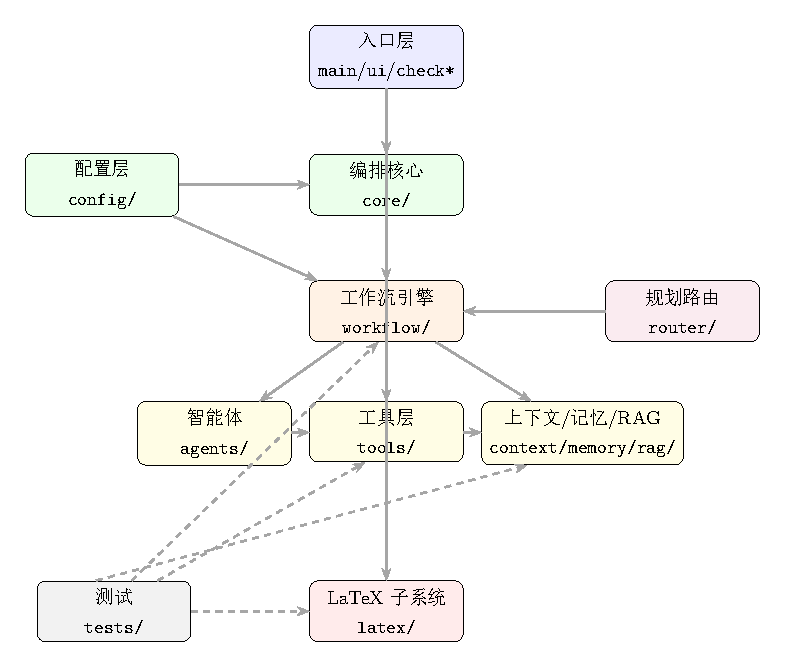
\includegraphics[width=\textwidth]{module_dependency_diagram.pdf}
\end{center}

\noindent\textbf{读图说明：}
\begin{itemize}[leftmargin=2em]
    \item \textbf{入口层}（\texttt{main.py}、\texttt{ui/}、\texttt{check*.py}）统一委托 \texttt{core/agent\_cli.py} 编排执行。
    \item \textbf{config/} 为全局配置源，被 \texttt{core/}、\texttt{workflow/}、\texttt{agents/} 等读取。
    \item \textbf{workflow/} 是执行中枢，调度 \texttt{agents/}、\texttt{tools/}，并借助 \texttt{context/}、\texttt{memory/}、\texttt{rag/} 拼装 Prompt。
    \item \textbf{router/} 仅在 Plan 模式下介入，将用户任务分解为动态图后交给 \texttt{workflow/}。
    \item \textbf{latex/} 作为独立子系统，主要由 \texttt{tools/latex\_*} 与 \texttt{ui/ghost/} 调用。
    \item 虚线表示 \texttt{tests/} 对各个功能模块的验证依赖（测试调用，非运行时依赖）。
\end{itemize}

\subsection{主要目录作用速查}

\begin{longtable}{@{}p{0.22\textwidth}p{0.36\textwidth}p{0.30\textwidth}@{}}
\toprule
\textbf{目录} & \textbf{作用} & \textbf{主要依赖} \\
\midrule
\endhead
\texttt{config/} & 环境变量、工作流 JSON、上下文 Profile、Planner Schema & 无（被各层读取） \\
\texttt{core/} & 消息协议、WorkflowState、TeXAgentCLI 编排入口 & \texttt{config/}, \texttt{workflow/} \\
\texttt{workflow/} & JSON/TaskPlan $\rightarrow$ LangGraph 图编译与执行 & \texttt{config/}, \texttt{agents/}, \texttt{tools/} \\
\texttt{agents/} & LLM 智能体（Simple/Multi/Reflection 等） & \texttt{core/}, \texttt{tools/} \\
\texttt{tools/} & 可插拔工具（arXiv、PDF、LaTeX、RAG 等） & \texttt{latex/}, \texttt{rag/}, \texttt{memory/} \\
\texttt{context/} & GSSC 上下文流水线，拼装 Agent Prompt & \texttt{config/}, \texttt{memory/} \\
\texttt{memory/} & 分支记忆、用户画像持久化 & \texttt{core/} \\
\texttt{rag/} & ChromaDB 向量检索管道 & \texttt{config/} \\
\texttt{router/} & Plan 模式 MAS 任务分解与图生成 & \texttt{config/}, \texttt{workflow/} \\
\texttt{latex/} & LaTeX 项目索引、L1/L2/L3 诊断修复、Ghost 窗口 & 系统 TeX 工具链（chktex/latexmk） \\
\texttt{ui/} & Web 聊天 UI、Overleaf 编辑器、Ghost 浮层 & \texttt{core/}, \texttt{latex/}, \texttt{rag/} \\
\texttt{cli/} & 终端 REPL 命令注册与分支管理 & \texttt{core/} \\
\texttt{utils/} & 日志、并发、回复格式化、取消控制等 & \texttt{config/} \\
\texttt{tests/}、\texttt{test/} & pytest 测试与演示脚本；详见测试文档 & 被测模块 \\
\bottomrule
\end{longtable}
